\chapter{Redes}
\section{Introducción, OSI vs TCP/IP}
Durante la asignatura de redes estudiamos el modelo OSI, sin embargo durante ésta asignatura nos centraremos en el estudio del modelo TCP/IP.\\

El modelo de Internet (TCP/IP) fue desarrollado en 1972 por el Departamento de Defensa de los Estados Unidos como una solución a un problema práctico de ingeniería.
\begin{figure}[H]
    \centering
    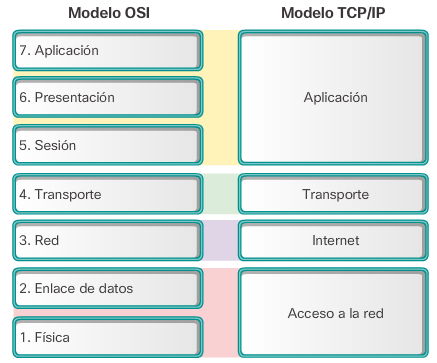
\includegraphics{img/OSIvsTCPIP.png}
    \caption{Comparativa de las capas de los modelos}
\end{figure}

En cambio, el modelo OSI(Open System Interconnection) fue propuesto como una solución teórica a los problemas de incompatibilidad entre redes.\\

Hoy en día es el modelo TCP/IP el que realmente se usa.
\section{Protocolo IPv4}
\begin{figure}[H]
    \centering
    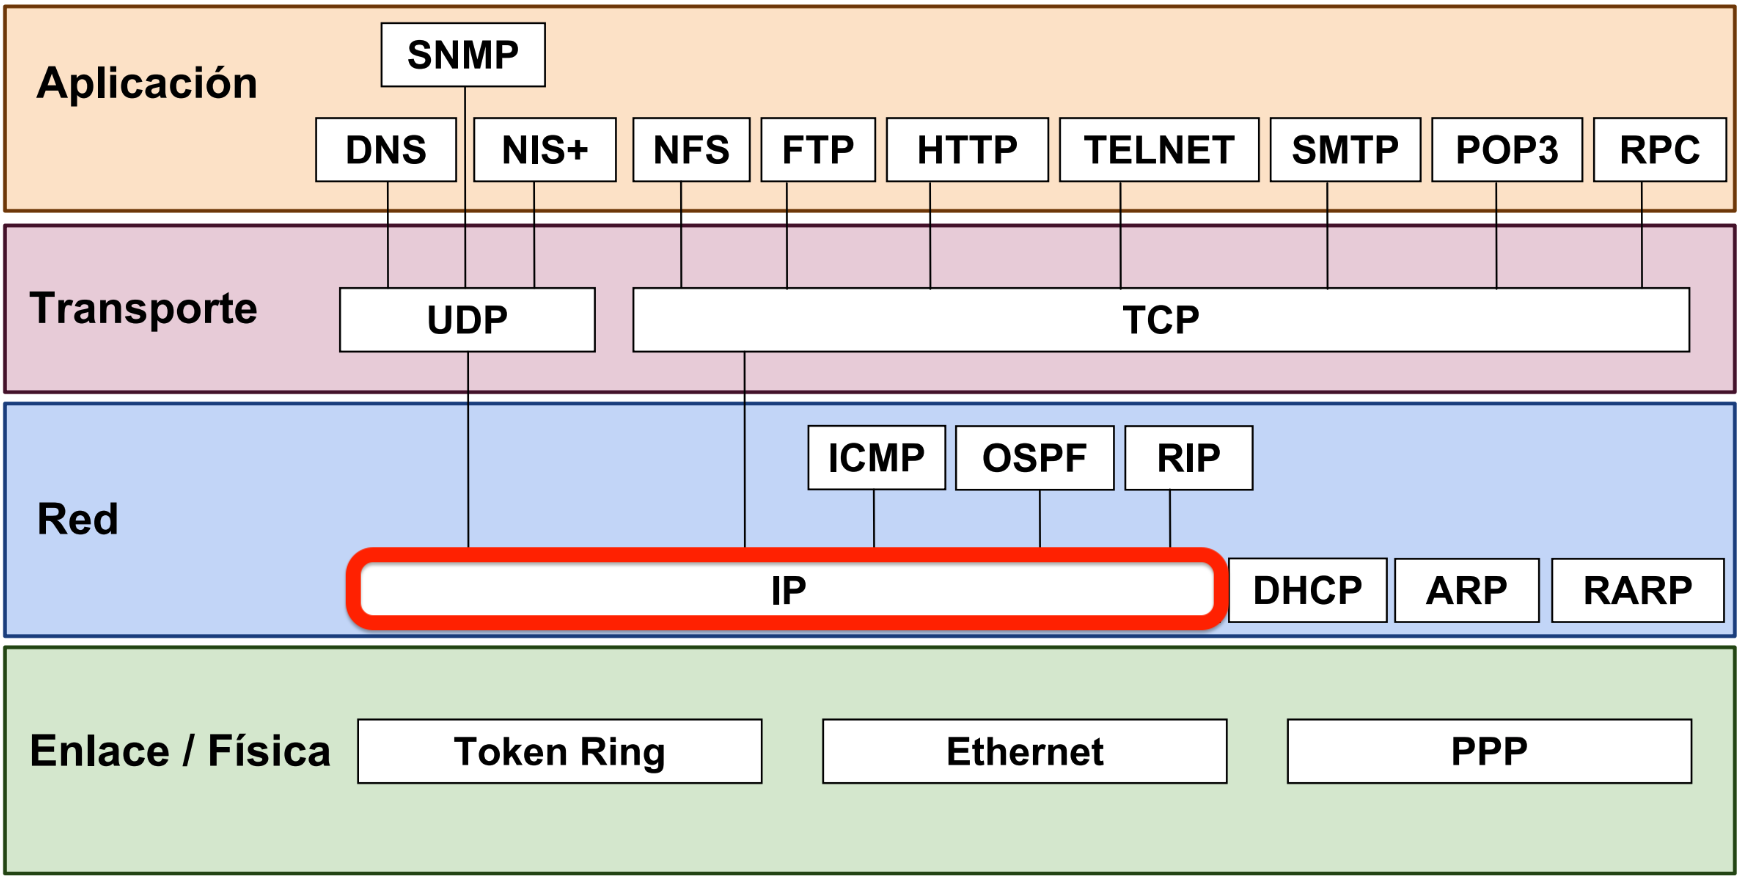
\includegraphics[width=0.7\textwidth]{img/IP.png}
\end{figure}
IP (Internet Protocol) es un protocolo de comunicación de datos digitales que transfiere paquetes a través de distintas redes físicas. Sus funciones básicas son:
\begin{itemize}
\item Encaminamiento: Saber por dónde tiene que enviar un mensaje.
\item Direccionamiento: Cómo nombrar las máquinas que están dentro de la red.
\item Fragmentación y Reensamblado: Traducir las tramas entre tecnologías distintas.
\end{itemize}
El protocolo IP es no orientado a conexión y no fiable, ésto quiere decir:
\begin{itemize}
    \item No detecta paquetes erróneos.
    \item No recupera paquetes perdidos.
    \item No garantiza que los paquetes lleguen en orden.
    \item No garantiza la detección de paquetes duplicados.
\end{itemize}
\subsection{Formato del mensaje IP}

El datagrama IP está formado por una cabecera IP seguida de un campo de datos. La cabecera para IPv4 es de la siguiente manera.

\begin{figure}[h]
\centering
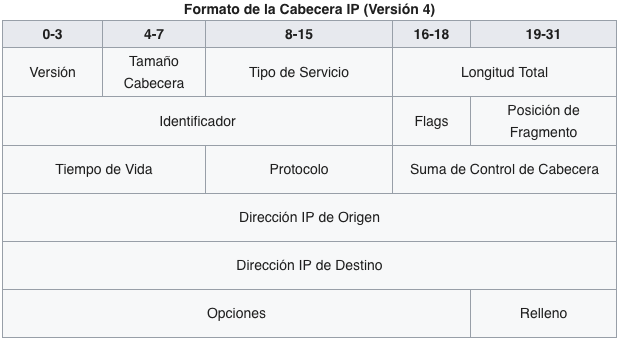
\includegraphics[width=0.85\textwidth]{img/datagramaIPv4.png}
\end{figure}

El campo opciones puede indicar:
\begin{itemize}
\item Encaminamiento desde el origen: lista de los encaminadores hasta llegar al destino. Usado para depuración o para saturar redes.
\item Registro de ruta: Cuando el datagrama llega al destinatario, tiene una lista de todos los routers por los que ha pasado.
\item Salto de tiempo: Cada router pone una marca de tiempo, se usa para medir el rendimiento de la red.
\end{itemize}

\subsection{Direccionamiento}

Una dirección IP es un número que identifica a una Interfaz en red  de un dispositivo que utilice el protocolo IP. La dirección IP no debe confundirse con la dirección MAC, que es un identificador de 48 bits para identificar de forma única la tarjeta de red y no depende del protocolo de conexión utilizando la red.\\

Las direcciones IPv4 se expresan mediante un número binario de 32 bits y se suelen expresar como números de notación decimal: se dividen los 32 bits de la dirección en cuatro octetos. El valor decimal de cada octeto está comprendido en el intervalo de 0 a 255. Ejemplo: [10.128.1.253]\\

\textbf{Tipos de direcciones IP.}\\
Las direcciones se dividen en dos campos de longitud variable: NetID (que identifica la red) y HostID (que identifica una máquina dentro de la red). Éstos rangos se indican mediante la máscara de red, que es un número que representa el número de bits de la NetID.

\begin{itemize}
\item Unicast: es el concepto más común en IP, se utiliza para un sólo dispositivo. [ej. 147.96.2.4]
\item Multicast: se utiliza para un grupo de receptores interesados. Se pueden utilizar direcciones comprendidas entre 224.0.0.0 - 239.255.255.255. [ej. 239.5.27.2]
\item Broadcast
	\begin{itemize}
	\item Limitada: usada para enviar a todas las máquinas de mi red LAN. [ej. 255.255.255.255]
    \item Dirigida: usada para enviar a todas las máquinas de una determinada red. [ej. 147.96.255.255]
	\end{itemize}
\item Anycast: envía el datagrama a la máquina más cercana de un grupo.
\end{itemize}

La direción IP debe ser única. Es la organización IANA quien se encarga de asignar las direcciones IP. Inicialmente se organizaron las direcciones IP en clases.

\begin{figure}[h]
\centering
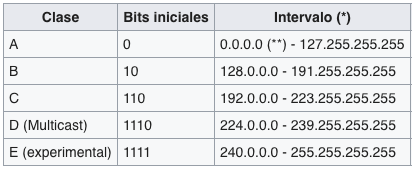
\includegraphics[width=0.65\textwidth]{img/clasesIP.png}
\end{figure}

El principal problema de esta forma de organización es el desperdicio de direcciones, por ello actualmente se utiliza una organización sin clases (CIDR).
\subsubsection{CIDR}
Classless Interdomain Routing, permite un uso más eficiente de las direcciones IP mediante la utilización de bloques de tamaños arbitrarios.\\

La notación CIDR permite expresar fácilmente las direcciones IP:\\

Consta de una direccion IPv4 de 32 bits seguida de una barra y un número, que indica el número de bits que identifican al bloque.\\

{\centering
    \textbf{122.233.2.1/24}\\
}


Ésta dirección indica que los primeros 24 bits de la dirección son los que identifican al bloque (Prefijo de red), y los otros 8 menos significativos son los que identifican al host.\\
\subsubsection{Direcciones reservadas}
El \textbf{identificador de host} tiene dos excepciones, según el valor de sus bits:
\begin{enumerate}
    \item \textbf{Todo a ceros:} indica que se trata de la dirección que identifica a la red (no de ninguna máquina), por tanto nunca se puede utilizar como dirección de destino.
    \item \textbf{Todo a unos:} indica que se trata de una dirección de broadcast, y al usarse como dirección de destino enviará el paquete a todas las máquinas de la red local.
\end{enumerate}
A parte, existen otras direcciones reservadas:
\begin{itemize}
  \item \textbf{10.x.x.x} red privada de clase A.
  \item \textbf{172.16.0.0 - 172.31.255.255} son 16 redes privadas de clase B.
  \item \textbf{192.168.x.x} son 256 redes privadas de clase C
  \item \textbf{127.x.x.x} Direcciones de Loopback (reenvían los paquetes a la misma máquina)
  \item \textbf{224.0.0.xxx} son direcciones multicast reservadas, por ejemplo:
  \begin{itemize}
      \item \textbf{224.0.0.1} Todos los hosts.
      \item \textbf{224.0.0.2} Todos los routers.
  \end{itemize}
\end{itemize}

%ARP
\section{Protocolo ARP}
\begin{figure}[H]
    \centering
    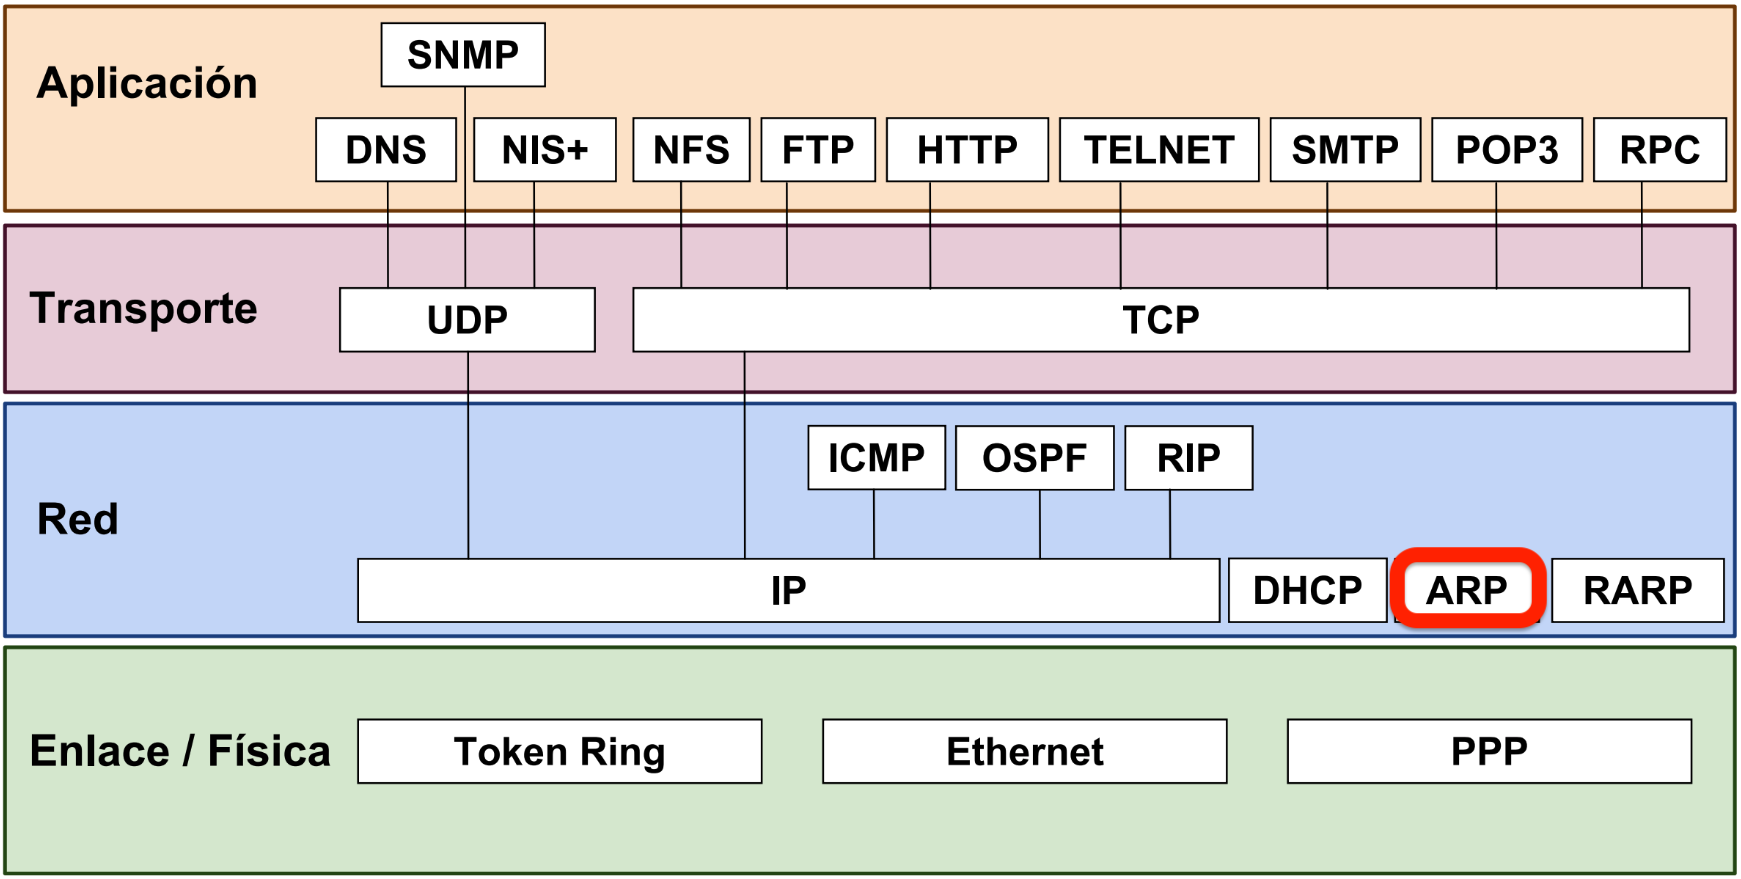
\includegraphics[width=0.7\textwidth]{img/ARP.png}
\end{figure}
Un datagrama IP tiene la siguiente forma.

\begin{table}[h] \centering \begin{tabular}{|c|c|}
\hline Cabecera IP & Datos \\ \hline \end{tabular}
\end{table}
A la hora de ser enviado, se encapsula \textbf{dentro del campo de datos} de otra trama más grande, la trama ARP.

\begin{table}[h] \centering \begin{tabular}{|l|c|c|l|l|}
\hline MAC Destino & MAC Origen & Protocolo & \textbf{Datos} & CRC \\ \hline \end{tabular}
\end{table}

ARP se encarga de encontrar la dirección MAC que corresponde a una determinada dirección IP. Para ello se envía un paquete (ARP request) a la dirección de difusión de la red (broadcast, MAC = FF FF FF FF FF FF) que contiene la dirección IP por la que se pregunta, y se espera a que esa máquina responda (ARP reply) con su dirección MAC.\\

Cada máquiena mantiene una tabla ARP en la que guarda las direcciones IP de las últimas máquinas con las que ha conectado, junto con su dirección MAC.

%ICMP
\newpage
\section{Protocolo ICMP}
\begin{figure}[H]
    \centering
    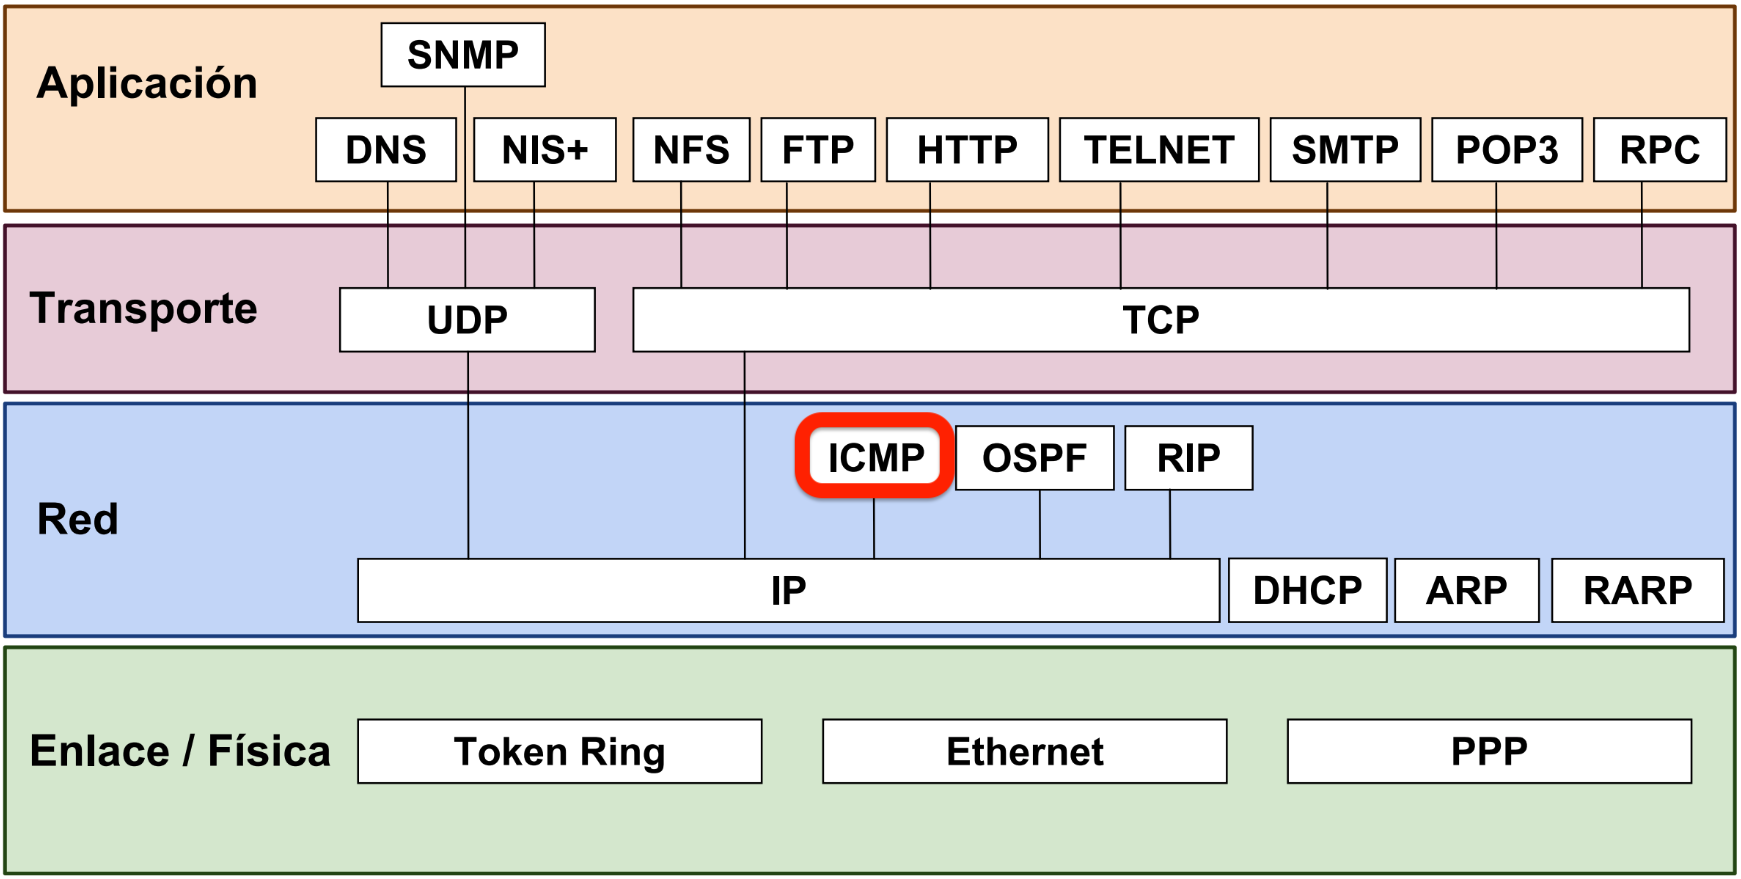
\includegraphics[width=0.7\textwidth]{img/ICMP.png}
\end{figure}
ICMP (Internet Control Message Protocol) es un protocolo de mensajes que viajan dentro del datagrama IP. Se usa para enviar mensajes de error, indicando por ejemplo que un router o host no puede ser localizado. También puede ser utilizado para transmitir mensajes de información.
\\\\
Algunos tipos de mensajes ICMP:
\begin{itemize}
\item De información
	\begin{itemize}
	\item \textbf{Echo Reply}
	\item \textbf{Echo Request}
    \item Redirect
    \item Router Solicitation
    \item Router Advertisement
	\end{itemize}
\item De error
	\begin{itemize}
	\item Destination Unreachable
    \item Source Quench
    \item Time Exceeded
    \item Parameter Problem
	\end{itemize}
\end{itemize}
\subsection{ECHO Request/Reply}
Como mensajes a destacar tenemos ECHO Request y ECHO Reply, que son los que utiliza la orden "ping" para comprobar la conexión.\\

Éstos mensajes tienen el siguiente formato:

\begin{table}[H]
\centering
\begin{tabular}{|c|c|c|}
\hline
\rowcolor[HTML]{9AFF99} 
Tipo = 0 & Código = 0  & Checksum \\ \hline
\rowcolor[HTML]{FDAAAA} 
\multicolumn{2}{|c|}{\cellcolor[HTML]{FDAAAA}{\color[HTML]{000000} Identificador}} & {\color[HTML]{000000} Número de secuencia} \\ \hline
\rowcolor[HTML]{FDAAAA} 
\multicolumn{3}{|c|}{\cellcolor[HTML]{FDAAAA}Datos :::}  \\ \hline
\end{tabular}
\end{table}
\begin{itemize}
    \item \textbf{Identificador:} Permitte establecer correspondencia entr solicitud (Request) y respuesta (Reply); ambos con el mismo identificador.
    \item \textbf{Secuencia:} También se utiliza para establecer la correspondencia entre solicitud y respuesta, cuando se envían varios Echo Requests consecutivos con el mismo identificador.
    \item \textbf{Datos:} Un número determinado de bytes aleatorios.
\end{itemize}

%DHCP
\newpage
\section{Protocolo DHCP}
\begin{figure}[H]
    \centering
    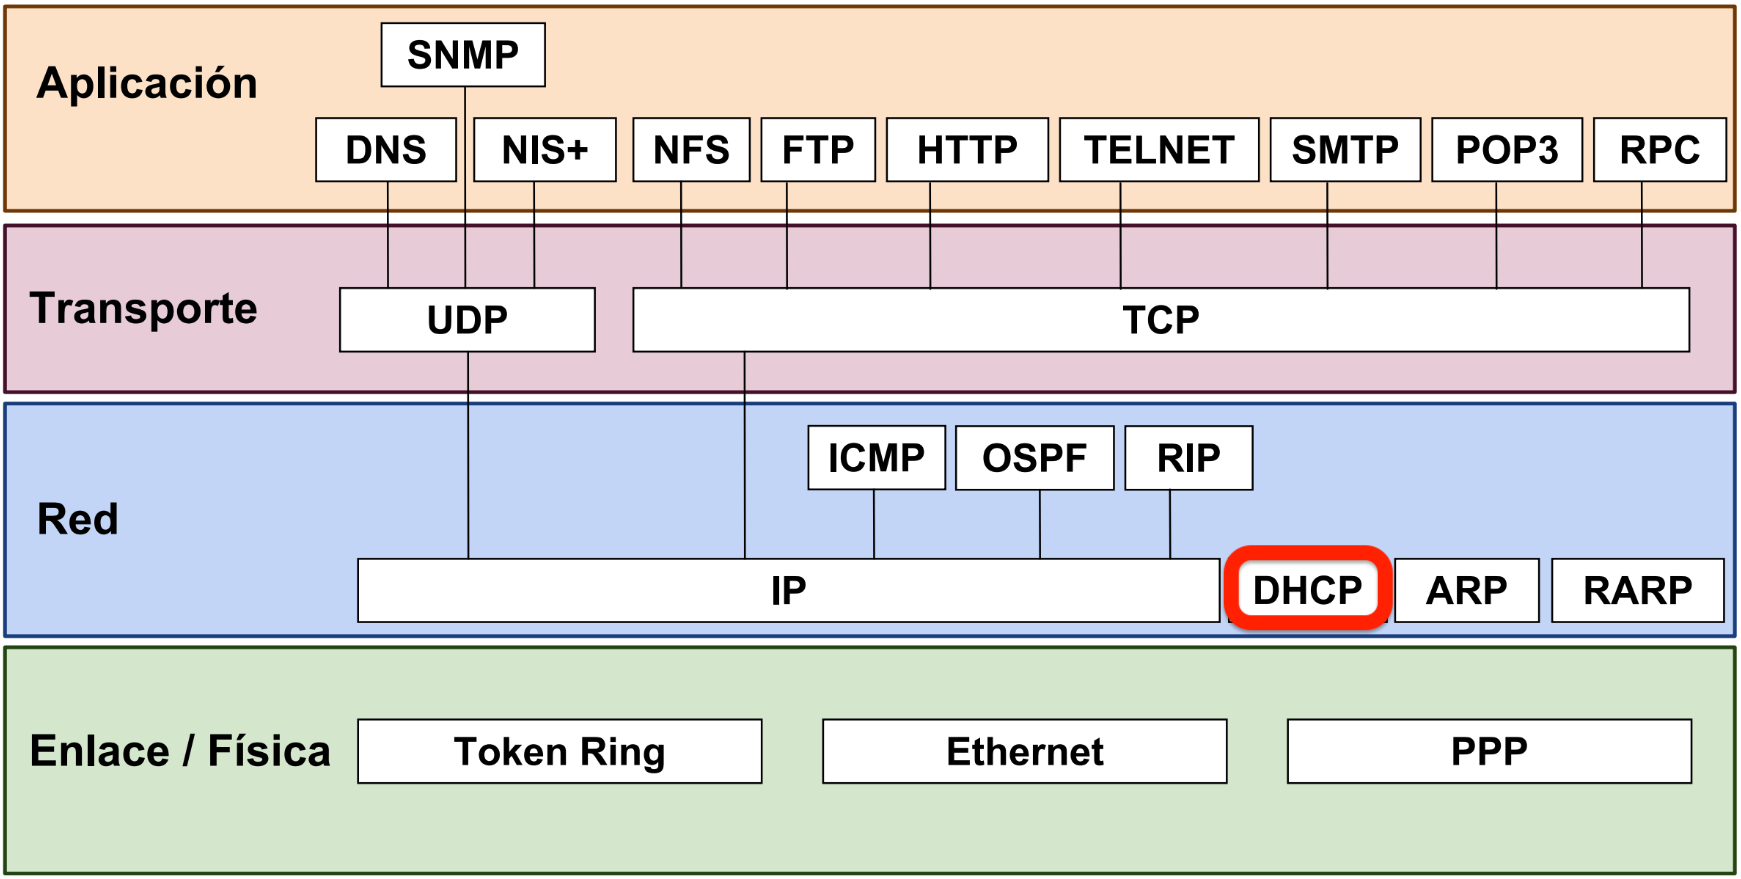
\includegraphics[width=0.7\textwidth]{img/DHCP.png}
\end{figure}

DHCP (Dynamic Host Configuration Protocol) es un protocolo que permite la configuración dinámica de direcciones IP y máscaras de red, router predeterminado, servidor DNS, y otros parámetros de configuración de red.\\

Este servidor posee una lista de direcciones IP dinámicas y las va asignando a los clientes conforme éstas van quedando libres, sabiendo en todo momento quién ha estado en posesión de esa IP, cuánto tiempo la ha tenido y a quién se la ha asignado después. Así los clientes de una red IP pueden conseguir sus parámetros de configuración automáticamente.\\

Algunas de sus \textbf{características} son:
\begin{itemize}
    \item Es un protocolo de red de tipo \textbf{cliente/servidor} sobre UDP en los puertos 67 (servidor) y 68
(cliente).
    \item Tiene un mecanismo de \textbf{control de errores} basado en sumas de comprobación, temporizadores y retransmisiones.
    \item Puede proveer de una servidor \textbf{TFTP} al dispositivo cliente. TFTP se utiliza para transferir pequeños archivos entre ordenadores en una red, como imágenes de arranque.
    \item En redes grandes con muchos enlaces, un servidor DHCP es ayudado por \textbf{DHCP relay agents} situados en routers intermedios. Estos agentes retransmiten los mensajes entre cliente y servidor situados en distintas subredes.
\end{itemize}
\subsection{Mensajes DHCP}
Estos son algunas de las operaciones que permite el protocolo.
\begin{itemize}
    \item DHCPDISCOVER: Mensaje del cliente (broadcast) para descubrir los servidores disponibles (puede contener la última dirección IP asignada).
    \item DHCPOFFER: Respuesta de los servidores, con una oferta de parámetros de configuración. Puede
    recibirse más de una.
    \item DHCPREQUEST: Petición de oferta del cliente (broadcast, para notificar a todos los servidores) o extensión del tiempo de cesión. El servidor seleccionado se especifica en una opción (Server Identifier, código 54).
    \item DHCPACK: Mensaje de confirmación (broadcast) y cierre desde el servidor hacia el cliente indicando los parámetros definitivos.
    \item DHCPRELEASE: Mensaje del cliente para informar al servidor de que ha finalizado el uso de
    la dirección IP.
\end{itemize}
\subsection{Datagrama DHCP}
\begin{figure}[H]
    \centering
    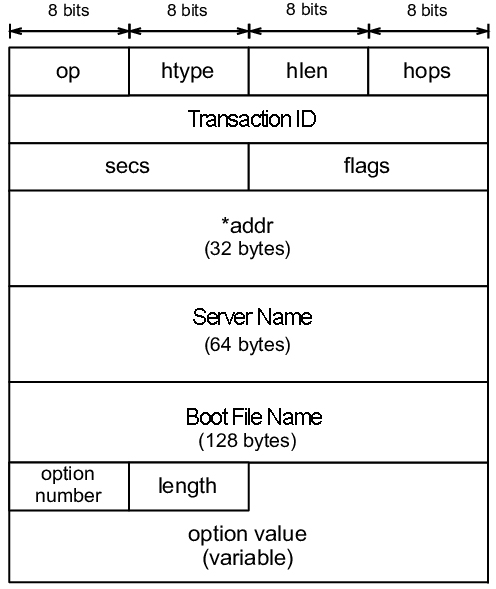
\includegraphics[width=0.5\textwidth]{img/DHCPformat.jpg}
    \caption{*addr: se guardan algunas direcciones como las de cliente y servidor.}
\end{figure}
%TCP
\newpage
\section{Protocolo TCP}
\begin{figure}[H]
    \centering
    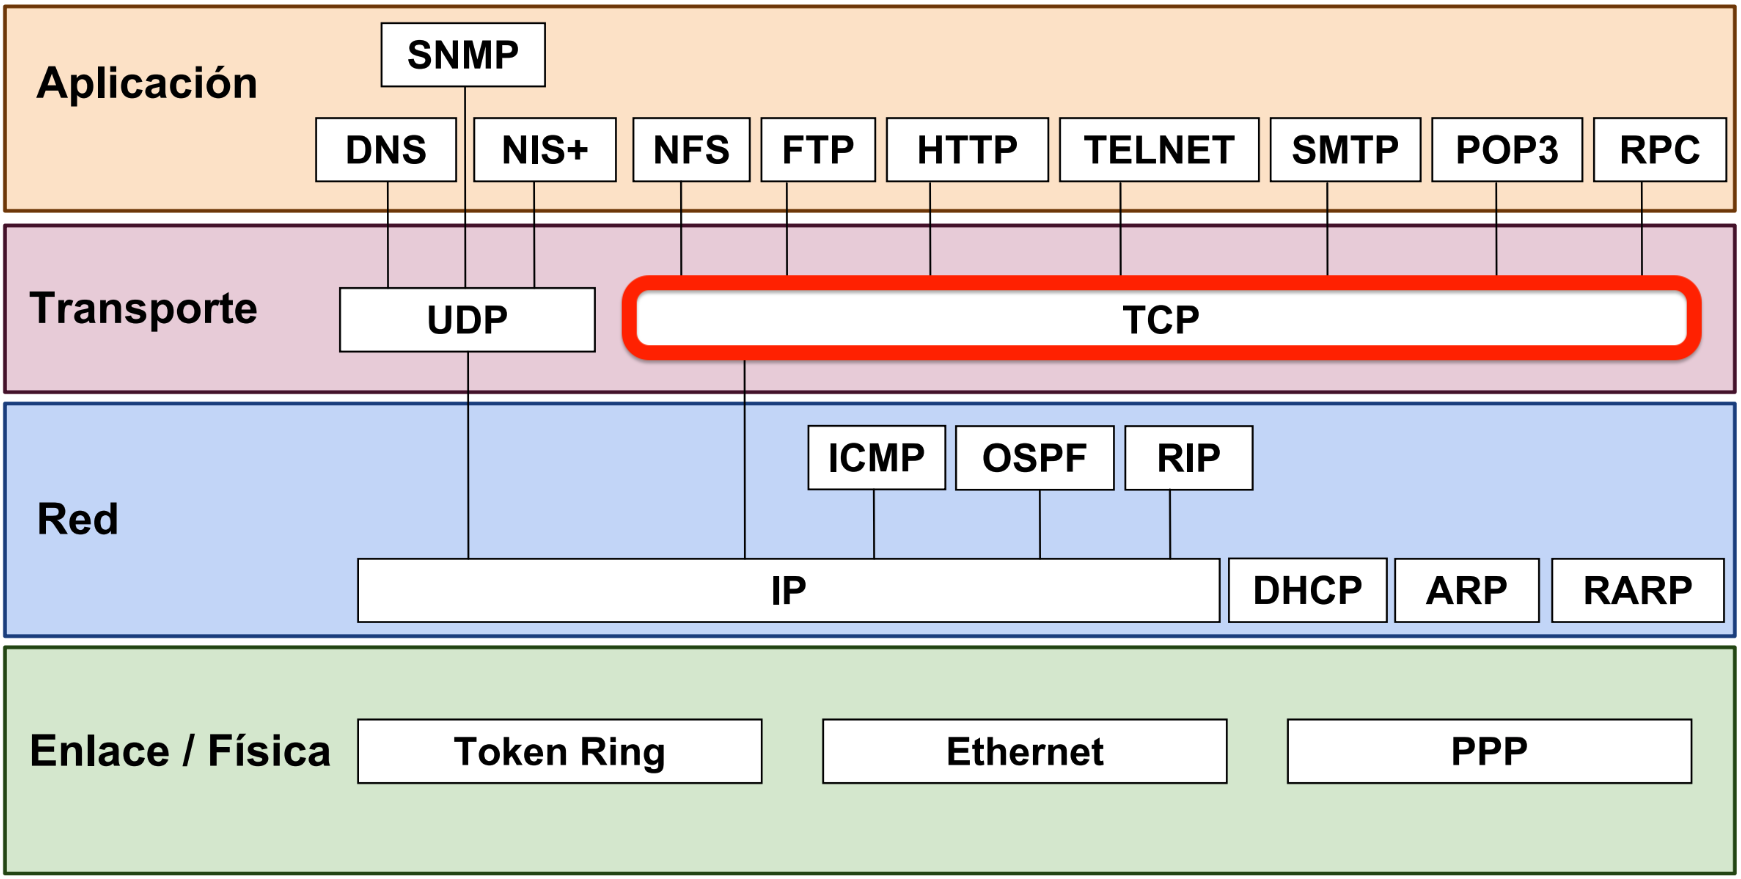
\includegraphics[width=0.7\textwidth]{img/TCP.png}
\end{figure}
TCP (Transmission Control Protocol) es un protocolo de transporte fiable y orientado a conexión (a diferencia de UDP, que es no fiable y no orientado a conexión). También proporciona un mecanismo para distinguir distintas aplicaciones dentro de una misma máquina, a través del concepto de puerto.

\subsubsection{Características de TCP}
\begin{itemize}
    \item Reordena los segmentos procedentes del protocolo IP y permite comenzar y finalizar la comunicación de forma consensuada entre ambas máquinas. \textbf{Orientado a conexión}.
    \item Monitorea el flujo de datos y así evita la saturación de la red. \textbf{Ventana Deslizante}.
    \item Permite que los datos se formen en segmentos de longitud variada para "entregarlos" al protocolo IP.
    \item Sirve para establecer la comunicación entre procesos de distintas máquinas. \textbf{Puertos}.
    \item Permite \textbf{multiplexar} los datos, es decir, que la información que viene de diferentes fuentes pueda circular simultáneamente por el mismo medio.
\end{itemize}
\subsection{Datagrama TCP}
\begin{figure}[H]
    \centering
    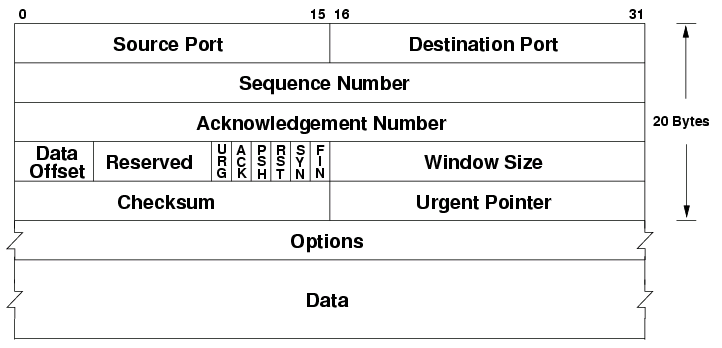
\includegraphics[width=0.9\textwidth]{img/TCPformat.png}
    \caption{Se divide en dos partes: datos (Data) y cabecera (Resto de campos).}
\end{figure}
\begin{itemize}
    \item \textbf{Source/Destination Port}: Identifican ambos extremos de la conexión.
    \item \textbf{Sequence/Acknowledgement Number}: Números de secuencia y confirmación expresados en bytes.
    \item \textbf{Reserved}: No se usa y se pone a 0.
    \item \textbf{Data offset}: Longitud de la cabecera.
    \item \textbf{Flags}
    \begin{itemize}
        \item URG: El segmento transporta datos urgentes (URG=1) desde el primer byte hasta el nº de byte especificado en el campo puntero urgente. TCP notifica a la aplicación de los datos urgentes (mediante la señal SIGURG), y ésta se encarga de tratarlos.
        \item ACK: El segmento contiene un número de confirmación válido (ACK=1). Todos los segmentos de una conexión TCP, excepto el primero, llevan ACK=1.
        \item PSH: Los datos deben ser entregados inmediatamente a la aplicación (PSH=1), o pueden almacenarse en el buffer (PSH=0).
        \item RST: Utilizado para abortar una conexión.
        \item SYN: Utilizado en el establecimiento de la conexión y sincronizar los números de
secuencia iniciales.
        \item FIN: Utilizado en la finalización de la conexión.
    \end{itemize}
    \item \textbf{Window Size}: Tamaño de la ventana.
    \item \textbf{Checksum}: Suma de comprobación.
    \item \textbf{Urgent Pointer}: Puntero que identifica el último byte de datos urgentes.
    \item \textbf{Options}: Campo de opciones de longitud variable.
    \item \textbf{Data}: Campo de datos de longitud variable.
\end{itemize}
\subsection{Fases de conexión}
Ya sabemos que TCP es un protocolo orientado a conexión, ahora vamos a ver detenidamente como se comunican dos máquinas.
\subsubsection{Fase de Establecimiento}
\begin{figure}[H]
    \centering
    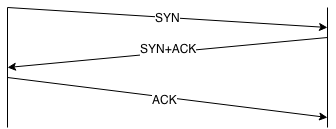
\includegraphics[width=0.55\textwidth]{img/SYN3.png}
\end{figure}
Una máquina (servidor) abre socket en un determinado puerto TCP y se queda a la escucha de nuevas conexiones (apertura pasiva).\\

Otra máquina (cliente) realiza una apertura activa de un puerto enviando un paquete SYN al servidor como parte de la negociación en tres pasos. En el lado del servidor se comprueba si el puerto está abierto, es decir, si existe algún proceso escuchando en ese puerto. En caso de no estarlo, se envía al cliente un paquete de respuesta con el bit RST activado, lo que significa el rechazo del intento de conexión.\\

En caso de que sí se encuentre abierto el puerto, el lado servidor respondería a la petición SYN válida con un paquete SYN/ACK. Finalmente, el cliente debería responderle al servidor con un ACK, completando así la negociación en tres pasos (SYN, SYN/ACK y ACK) y la fase de establecimiento de conexión. Es interesante notar que existe un número de secuencia generado por cada lado, ayudando de este modo a que no se puedan establecer conexiones falseadas (spoofing).\\


\begin{tcolorbox}[
title=SYN Flood,
colback=blue!5!white,
colframe=blue!75!black,
fonttitle=\bfseries]
Es una vulnerabilidad en el protocolo que consiste en enviar una gran cantidad de segmentos TCP con el flag SYN activado, saturando el servidor (ataque DoS), ya que asigna recursos a cada intento de conexión. Para evitarlos se puede:
\begin{itemize}
    \item Limitar el número de conexiones.
    \item Aceptar conexiones sólo de IP’s confiables.
    \item Retrasar la asignación de recursos usando SYN cookies.
\end{itemize}
\end{tcolorbox}

\subsubsection{Fase de Transferencia}
Durante la etapa de transferencia de datos, una serie de mecanismos claves determinan la fiabilidad y robustez del protocolo. Entre ellos están incluidos el uso del \textbf{número de secuencia} para ordenar los segmentos TCP recibidos y detectar paquetes duplicados, \textbf{checksums} para detectar errores, \textbf{temporizadores} para detectar pérdidas o retrasos y \textbf{ventanas deslizantes} para el control de flujo de datos.
\subsubsection{Fase de Finalización}
La fase de finalización puede realizarse de dos maneras:
\begin{itemize}
    \item \textbf{Finalización de 4 vías}:
\begin{figure}[H]
    \centering
    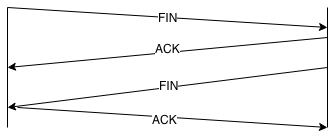
\includegraphics[width=0.55\textwidth]{img/FIN4.png}
\end{figure}
    \begin{enumerate}
        \item El cliente deja de enviar datos al servidor, y le envía un paquete con el flag FIN activado.
        \item El servidor le responde con un paquete con el flag ACK.
        \item Cuando el servidor deja de tener datos para enviar, envía otro paquete con el flag FIN.
        \item El cliente le responde con ACK, tras lo cual se cierra la conexión.
    \end{enumerate}
    \item \textbf{Finalización de 3 vías}:
\begin{figure}[H]
    \centering
    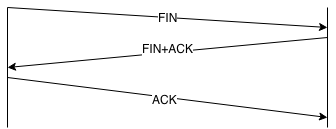
\includegraphics[width=0.55\textwidth]{img/FIN3.png}
\end{figure}
    \begin{enumerate}
        \item El cliente deja de enviar datos al servidor, y le envía un paquete con el flag FIN activado.
        \item El servidor le responde con un paquete con los flags FIN y ACK activados y deja de enviar datos.
        \item El cliente le responde con ACK, tras lo cual se cierra la conexión.
    \end{enumerate}

\end{itemize}
\subsubsection{Diagrama de estados}
\begin{figure}[H]
    \centering
    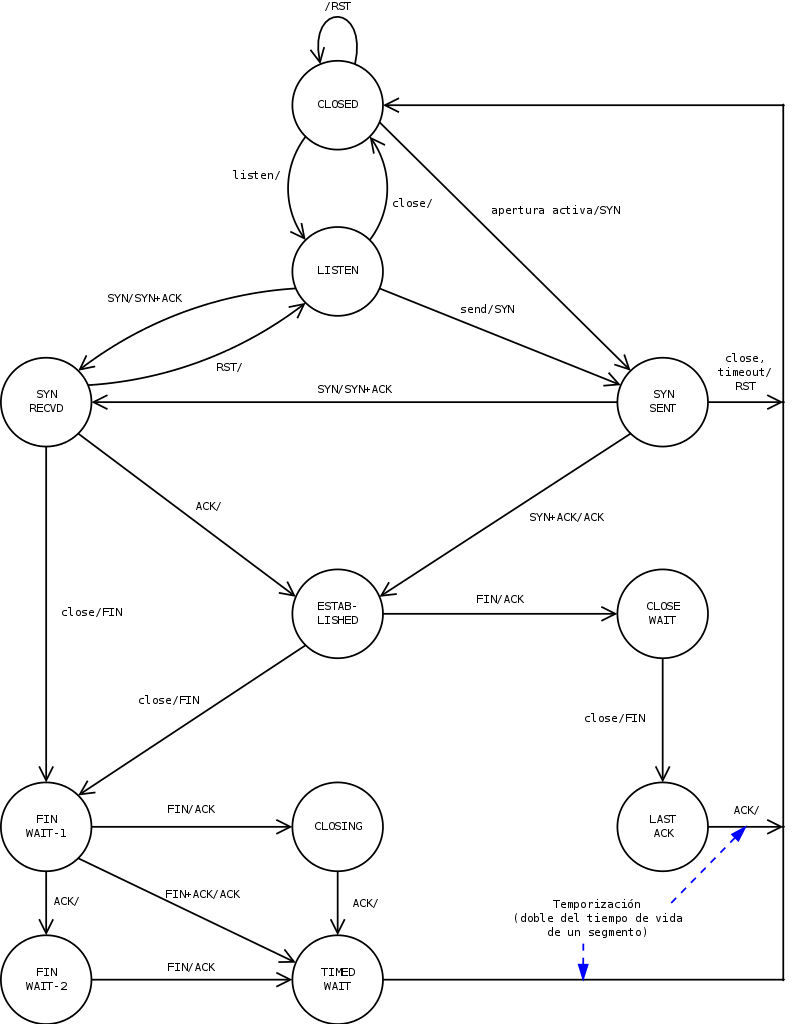
\includegraphics[width=0.98\textwidth]{img/EstadosTCP.png}
\end{figure}
\newpage
\subsection{Ventana deslizante}
TCP consigue transferencia fiable mediante el uso de la \textbf{ventana deslizante}.
\subsubsection{Parada y Espera vs. Ventana Deslizante}
En los protocolos de \textbf{parada y espera}, cuando el emisor envía un segmento, tiene que esperar a recibir un ACK antes de poder enviar el siguiente segmento.\\

Si después del timeout no llega el ACK, el emisor vuelve a enviar el segmento. Esto implica que un transmisor solo puede tener un elemento pendiente de reconocimiento, lo cual es bastante ineficiente.\\

Los protocolos de \textbf{ventana deslizante} por el contrario, pueden enviar varios segmentos sin esperar a recibir las confirmaciones de una en una.\\

La ventana deslizante permite:
\begin{itemize}
    \item La recepción de segmentos duplicados.
    \item La retransmisión de segmentos erróneos o perdidos.
    \item La recepción de segmentos fuera de orden.
\end{itemize}
\begin{figure}[H]
    \centering
    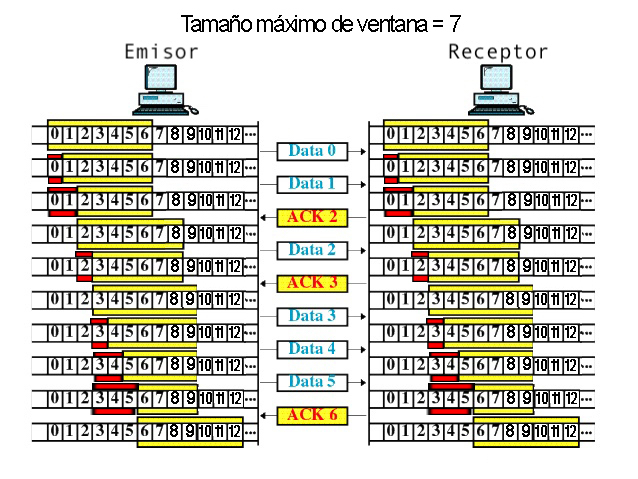
\includegraphics[width=\textwidth]{img/ventanasTCP.jpg}
    \caption{Intercambio de paquetes mediante ventana deslizante.}
\end{figure}
\subsubsection{Emisor}
\begin{itemize}
    \item Almacena los elementos pendientes de reconocimiento [marcados en rojo en el ejemplo]. El límite inferior de la ventana indica el primer segmento sin confirmar (si lo hay), o el siguiente segmento a enviar (si todos los segmentos están confirmados).
    \item Almacena también los elementos que pueden ser enviados [marcados en amarillo].
    \item El tamaño de la ventana siempre es igual al tamaño máximo [7 en el ejemplo]. Excepto cuando la aplicación no tiene tantos datos para enviar, en cuyo caso es menor.
\end{itemize}
\subsubsection{Receptor}
\begin{itemize}
    \item Almacena los elementos pendientes de ser consumidos por la aplicación [marcados en rojo en el ejemplo]. El límite inferior de la ventana indica el primer segmento sin ser consumido (si lo hay), o el siguiente segmento a recibir (si todos los segmentos están consumidos).
    \item Almacena también los elementos que pueden ser recibidos [marcados en amarillo].
    \item El tamaño de la ventana siempre es igual al tamaño máximo [7 en el ejemplo]. Excepto cuando la aplicación no tiene tantos datos para recibir, en cuyo caso es menor.
    \item Una vez los segmento son recibidos, el receptor envía un ACK, cuyo número indica el siguiente segmento a recibir.
    \item Para enviar los ACK se utiliza la técnica de \textbf{Piggybacking}, que consiste en incluir el ACK en otro segmento de datos que el receptor quiera enviar al emisor (ya que la comunicación es bidireccional).
\end{itemize}
\newpage
\subsection{Control de errores}
Vamos a ver cómo TCP resuelve algunas situaciones conflictivas.
\subsubsection{Recepción fuera de orden}
TCP controla la recepción de datos fuera de orden mediante confirmaciones (ACK) de la siguiente forma.
\begin{figure}[H]
    \centering
    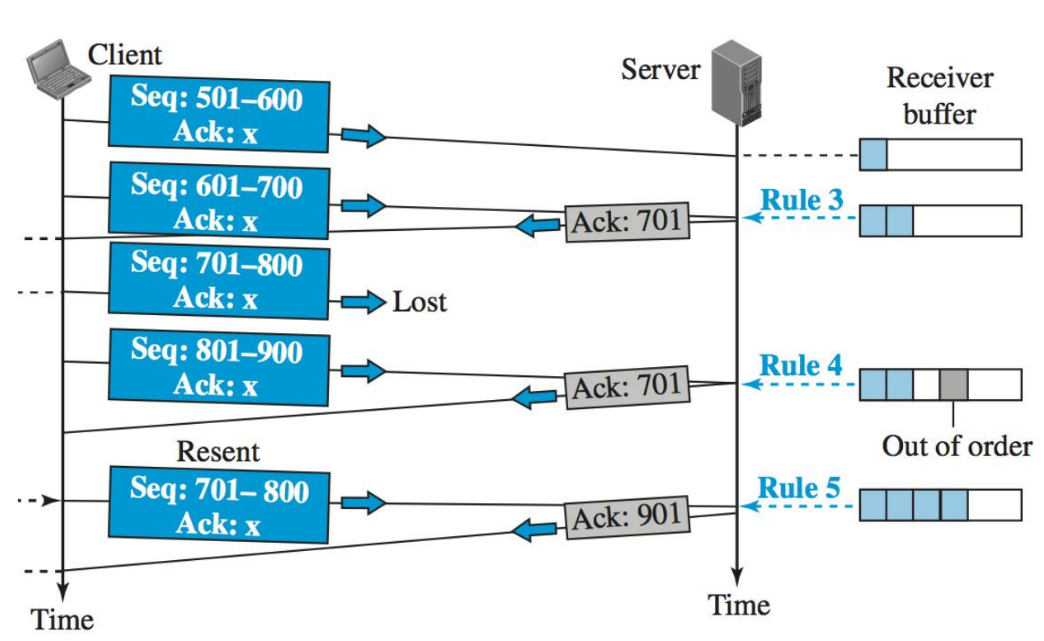
\includegraphics[width=\textwidth]{img/TCPooo.png}
    \caption{Recepción fuera de orden.}
\end{figure}
\begin{itemize}
    \item Si hay huecos, el receptor envía el ACK del primer hueco que tenga en el buffer.
    \item Si no hay huecos envía el ACK del siguiente segmento esperado.
    \item Los segmentos duplicados se confirman para prevenir pérdidas de ACK.
\end{itemize}
\subsubsection{Pérdida de un segmento}
¿Qué hacer cuando se pierde un segmento, o se recibe erróneamente? para ello TCP tiene dos \textbf{mecanismos de retransmisión}:
\begin{itemize}
    \item \textbf{Temporizador de retransmisión:} si el emisor tiene segmentos sin confirmar, los reenvía al finalizar el temporizador. Si hay varios segmentos sin confirmar, el emisor reenvía el primero de la ventana.
        \begin{figure}[H]\centering
        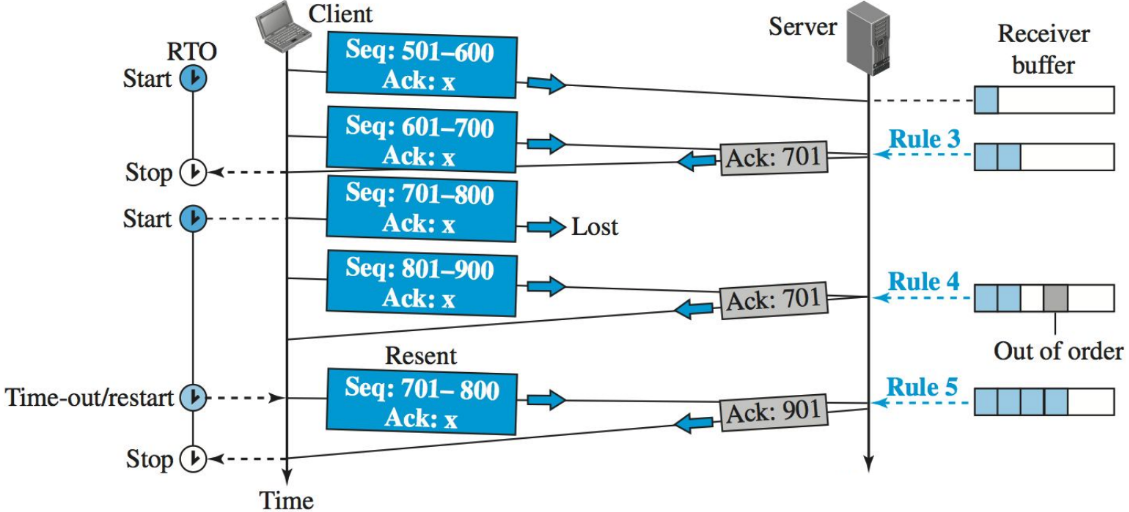
\includegraphics[width=\textwidth]{img/TCPTdRet.png}
        \caption{Temporizador de retransmisión.}\end{figure}
    \item \textbf{Retransmisión rápida:} si se reciben tres ACKs duplicados, el emisor reenvía el paquete.
        \begin{figure}[H] \centering
        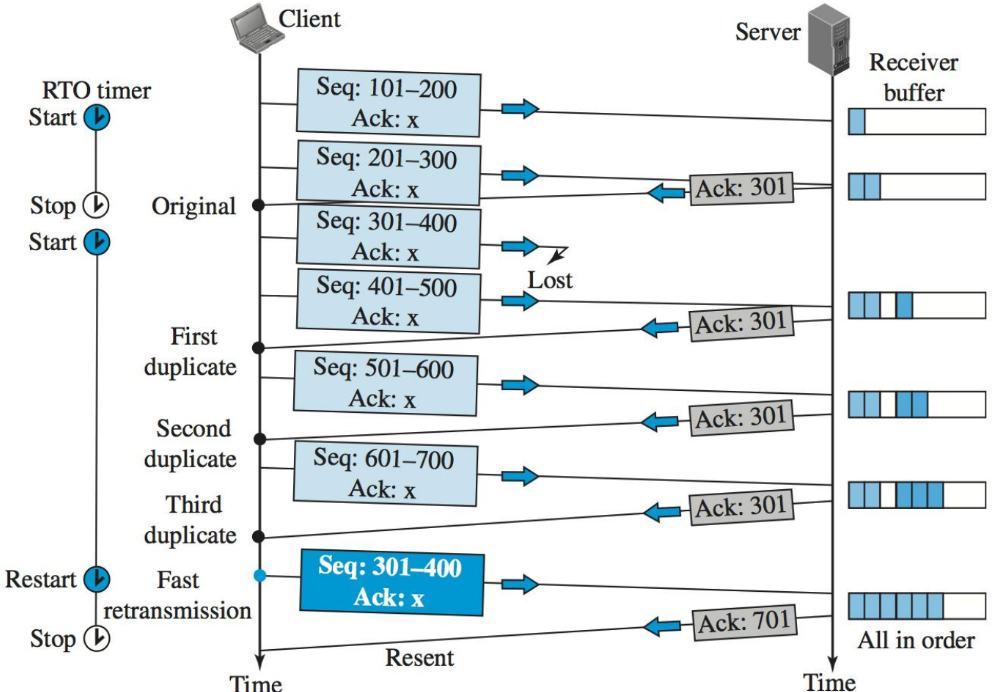
\includegraphics[width=\textwidth]{img/TCPRetRap.png}
        \caption{Retransmisión rápida.}\end{figure}
\end{itemize}
\newpage
\subsubsection{Pérdida de un ACK}
Con respecto a la pérdida de ACKs se pueden dar dos situaciones.
\begin{itemize}
    \item \textbf{No expira el temporizador de retransmisión:} el emisor sigue enviando paquetes, por lo que si el siguiente ACK confirma un segmento posterior, también confirma todos los anteriores.
        \begin{figure}[H]\centering
        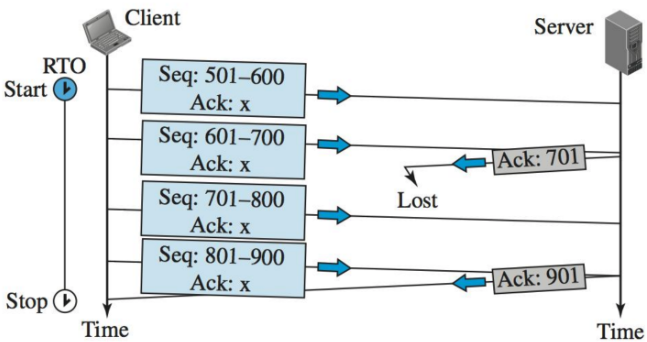
\includegraphics[width=\textwidth]{img/TCPACK1.png}
        \caption{No expira el temporizador de retransmisión.}\end{figure}
    \item \textbf{Expira el temporizador de retransmisión:} si el emisor no sigue enviando paquetes, cuando su temporizador de retransmisión expire, reenviará el paquete sin confirmar.
        \begin{figure}[H] \centering
        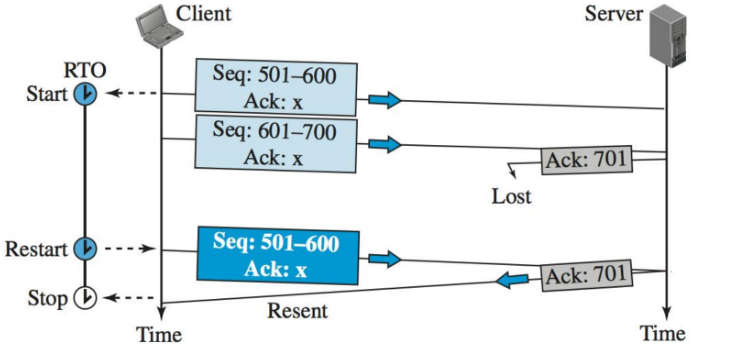
\includegraphics[width=\textwidth]{img/TCPACK2.png}
        \caption{Expira el temporizador de retransmisión.}\end{figure}
\end{itemize}


\newpage
\subsection{Temporizadores TCP}
TCP utiliza 4 temporizadores.
\begin{itemize}
    \item \textbf{Keepalive: }se utiliza para comprobar si un enlace está o no operativo. Cuando el temporizador expira (más de 2 horas, normalmente) envía una serie de señales \textit{keepalive}. Si no recive los ACK correspondientes, cierra la conexión.
    \item \textbf{TIMEWAIT: }en el cierre de conexión es el tiempo que espera la máquina que ha iniciado el cierre después de recibir el FIN (tanto en 3 como en 4 vías), para dar tiempo a la otra máquina a recibir el último ACK.
    \begin{figure}[H] \centering
    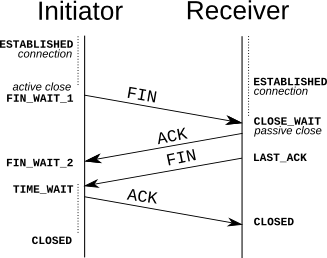
\includegraphics[width=0.5\textwidth]{img/TCP_TIMEWAIT.png}\end{figure}
    \item \textbf{Temporizador de persistencia: \label{tempers}}cuando el receptor advierte de un tamaño de ventana igual a 0, el emisor deja de enviar datos e inicia el temporizador de persistencia. El temporizador de persistencia se usa para proteger a TCP de una situación de interbloqueo que podría surgir si se pierde una actualización del tamaño de la ventana del receptor, y el emisor no puede enviar más datos hasta que reciba una nueva actualización del tamaño de la ventana del receptor. Cuando el temporizador expira, el emisor envía un pequeño paquete esperando un ACK, que le indique el nuevo tamaño de ventana.
    \item \textbf{Temporizador de retransmisión: }se utiliza cuando se espera un ACK del otro extremo. Veámoslo con más detalle.
\end{itemize}
\newpage
\begin{tcolorbox}[
title=Temporizador de retransmisión (TIMEOUT),
colback=cyan!5!white,
colframe=cyan!75!black,
fonttitle=\bfseries]
El tiempo de TIMEOUT se establece dinámicamente en función del tráfico de la red, y se pueden usar 3 algoritmos distintos para establecerlo.\\

El tiempo de ida y vuelta (\textbf{RTT}), es el tiempo transcurrido desde que se envía el
segmento hasta que se recibe el ACK. El RTT puede presentarse de tres formas distintas:
\begin{itemize}
    \item \textbf{RTT medido (RTTm): }es el RTT tal cual, por lo que puede experimentar grandes fluctuaciones. Por ejemplo si recibe un ACK acumulado, el RTTm se disparará.
    \item \textbf{RTT suavizado (RTTs): }es la media ponderada entre el RTTm y el último RTTS calculado. De forma que el primer RTTs = RTTm, y los siguientes valores dependen del RTTm actual y del RTTs anterior.
    \item \textbf{RTT desviación (RTTd): }Considera la variación del tiempo de ida y vuelta, y se calcula a partir del RTTm y del RTTs.
\end{itemize}

En éstos valores se basan los 3 \textbf{algoritmos} que puede usar el temporizador de retransmisión.
\begin{itemize}
    \item \textbf{Jacobson: }utiliza únicamente RTTs.
    \item \textbf{Jacobson/Karels: }mejora el anterior combinando RTTS y RTTD.
    \item \textbf{Karn: }se basa en el anterior se basa solo en ACKs de segmentos que fueron enviados solo una vez.
\end{itemize}
\end{tcolorbox}
\subsection{Control de flujo}
El control de flujo se utiliza para evitar desbordar el buffer del receptor cuando transmitimos muy rápido demasiados datos. Para ello TCP adaptará dinámicamente la ventana del emisor, dependiendo del tamaño de la ventana del receptor (anunciado cada ACK).\\

Si el receptor se queda sin espacio, su ventana tendrá tamaño = 0, y el emisor dejará de enviar datos. El emisor volverá a enviar datos de nuevo cuando el tamaño de la ventana del receptor vuelva a ser mayor que 0. Para saber el tamaño, utiliza el \underline{\hyperref[tempers]{temporizador de persistencia.}}

\newpage
\subsubsection{Síndrome de la ventana tonta}
Ocurre cunado o bien el servidor genera datos a un ritmo muy lento, o bien el cliente consume los datos a un ritmo muy lento.\\
\begin{tcolorbox}[colback=white]
Para evitar la ventana tonta en el \textbf{emisor} se inventó el \textbf{algoritmo de Nagle}:
\begin{itemize}
    \item Se envía el primer mensaje.
    \item Se espera a enviar los siguientes hasta que:
    \begin{enumerate}
        \item se recibe un ACK del receptor.
        \item se acumulan x bytes.
        \item expira el TIMEOUT.
    \end{enumerate}
\end{itemize}
\end{tcolorbox}
\begin{tcolorbox}[colback=white]
Para evitar la ventana tonta en el \textbf{receptor} se inventó el \textbf{algoritmo de Clark}:
\begin{itemize}
    \item Se anuncia tamaño de ventana 0 hasta que:
    \begin{enumerate}
        \item Se puede recibir un segmento completo.
        \item Se ha liberado la mitad del buffer de recepción.
    \end{enumerate}
\end{itemize}
\end{tcolorbox}


\subsection{Control de la congestión}
A diferencia del control de flujo, el \textbf{control de congestión} puede aparecer en cualquier punto de la red. Si un router no es capaz de gestionar todos los paquetes, empieza a descartar.\\

%TODO: revisar
El emisor controla el ritmo de envío según el ritmo al que recibe las confirmaciones, para ello utiliza la Ventana de congestión (CW).\\

En una situación ideal la ventana de recepción y la ventana de congestión tienen el mismo tamaño.\\

\subsubsection{Fases del control de la congestión}
\begin{itemize}
    \item La transmisión comienza con CW = 1
    \item Fase de arranque lento: el tamaño aumenta exponencialmente con cada segmento enviado hasta llegar a un umbral (SST).
    \item Fase de evitación de congestión: Cuando se confirman todos los segmentos de la ventana la CW aumenta en +1 (crecimiento lineal).
    \item Fase constante: si la CW alcanza el mismo tamaño que la ventana de flujo (RW), el tamaño se mantiene.
\end{itemize}
A partir de aqui pueden aparecer congestiones que se detectan de forma indirecta:
\begin{itemize}
    \item Se reciben 3 ACKs duplicados. Nivel de congestión leve...
    \item Expira el temporizador de retransmisión. Nivel de congestión elevado...
\end{itemize}
%%%%%%%%%%%%%% Dia 3 %%%%%%%%%%%%%%
\section{Servicios de Red: Filtrado de paquetes}
\subsection{Firewall y filtrado de paquetes}
Firewall filtra el trafico malicioso o indeseado entre Internet y una red privada.
Tipos de Firewall
\begin{itemize}
    \item De red
    \item De Host
    ---
    \item Se pueden distinguir en funcion de si tienen o no estado: Pueden determinar si el paquete esta intentando abrir una conexion nueva o pertenece a una ya existente.
    SPI (Stainfull packet Inspection)...
    \item En función de la capa: Filtran el trafico en funcion del contenido de las cabeceras de los segmentos de red. Consideran:
    \begin{itemize}
        \item Direcciones
        \item Puertos   
        \item Tamaño de los datos
    \end{itemize}

    \item Firewalls de aplicación: consideran informacion no solo de las cabeceras si no de los datos(que normalmente pertenecen a protocolos de aplicación como http). Este tipo de firewalls se dice que realizan DPI (Deep packet inspection).
\end{itemize}

\subsection{Netfilter/Iptables}
Netfilter/iptables son las herramientas de filtrado de paquetes de Linux.
Es a nivel de red y con estado. Netfilter es una herramienta del kernel de Linux proporciona filtrado de paquetes y modificación de paquetes.
\\
\textbf{Cadena}: lista ordenada de reglas que se aplican sobre los paquetes en distintos puntos del proceso del paquete.
Tablas y cadenas predefinidas:
\begin{itemize}
    \item Tabla filter: es la tabla por defecto
        Contiene tres cadenas, que clasifica los paquetes:
        \begin{itemize}
            \item INPUT: paquetes recibidos.
            \item OUTPUT: paquetes generados.
            \item FORWARD: paquetes que atraviesan el sistema.
        \end{itemize}
    
    \item Tabla NAT: Reescribe direcciones y contiene tres cadenas.
            \begin{itemize}
                \item PREOUTING:
                \item POSTROUTING: se aplica a paquetes justo antes de ser enviados, modifica la direccion de origen de los paquetes.
                \item OUTPUT: similar a la cadena homonima de la tabla filter.
            \end{itemize}
    \item Tabla Mangle: contiene las cinco cadenas anteriores.
    
    \begin{figure}[H]
        \centering
        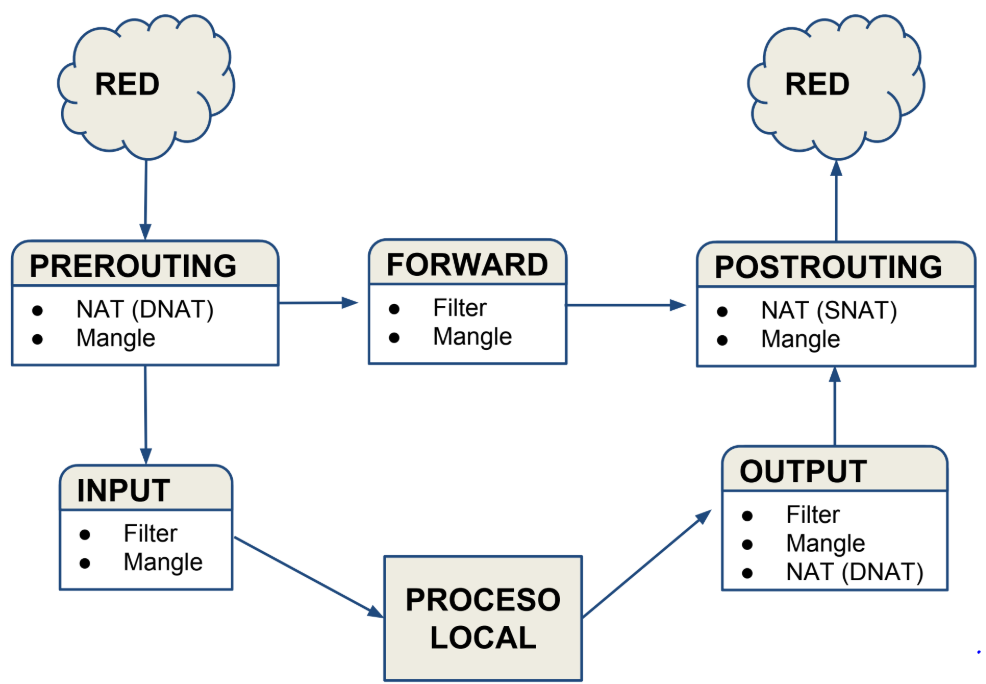
\includegraphics[width=0.8\textwidth]{img/GraficoCadenas.PNG}
        \caption{Diagrama de cadenas}
    \end{figure}
    
    Definición de Reglas: las reglas se pueden definir según la información del paquete o según el estado de la conexión. Debe incluir la cadena a la que se añade la regla y un objetivo.
    \begin{figure}[H]
        \centering
        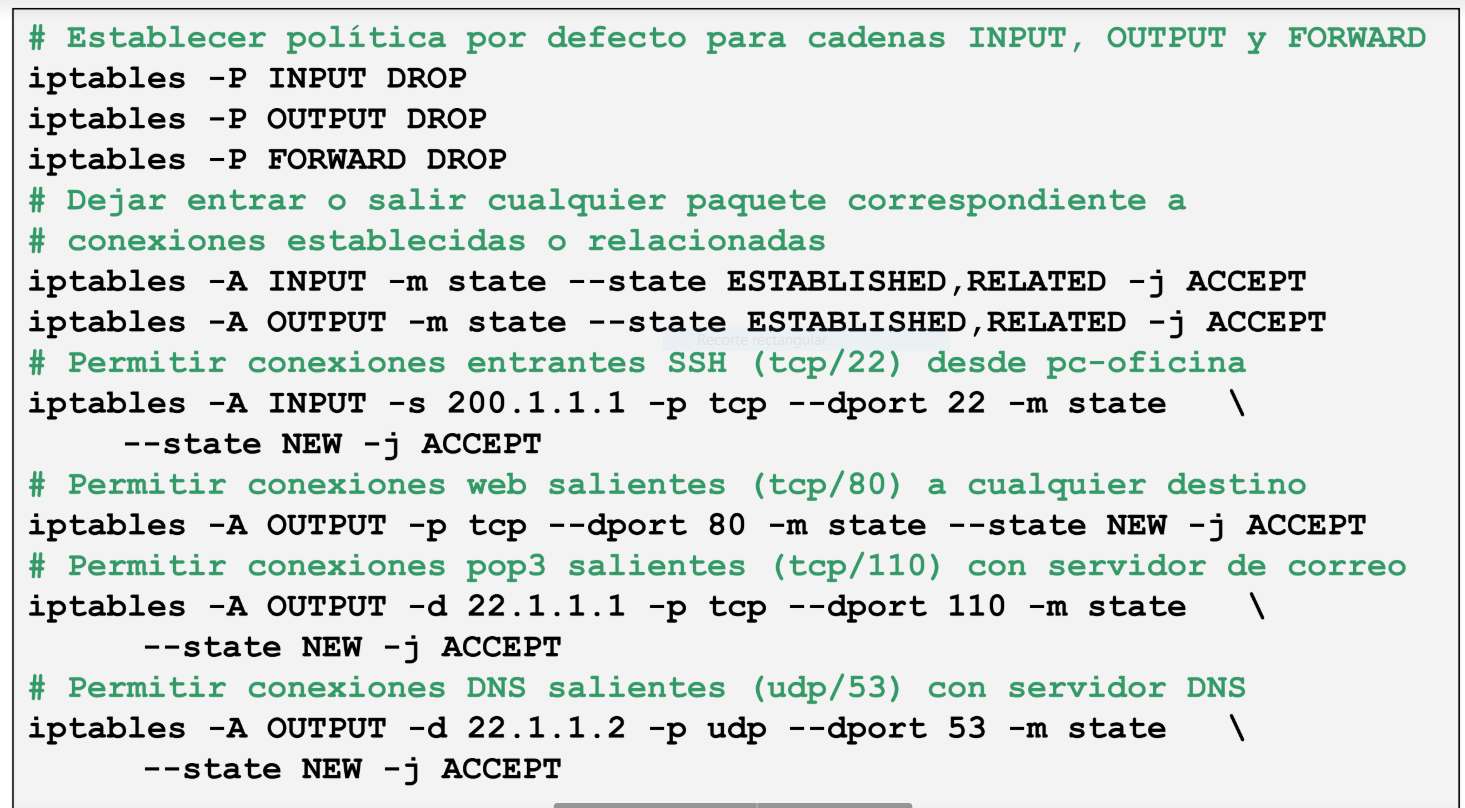
\includegraphics[width=\textwidth]{img/EjemplosReglas.PNG}
        \caption{Ejemplos de reglas}
    \end{figure}
    \subsubsection{NAT}
    NAT: Network Address Translation: permite dar acceso a Internet a máquinas en redes privadas realizando traducciones. Para ello se utiliza Masquerading: traduce la dirección privada a la dirección pública asignada al router. Para los mensajes entrantes el router tiene una tabla con unas traducciones que depende del \textbf{número de puerto} asignado con el router.
    
    Port forwarding, servidores virtuales: hace una traduccion de direcciones de red destino. Todos los servidores utilizan la misma ip publica (La del router), la diferencia con el anterior caso el que la tabla se define previamente y no de forma dinámica.
\end{itemize}

%%%%%%%%%%%%%%%%%%%%%%%%%%%%%%%%%%%%%%%%%%%%%%%%%%%
\section{DNS}
Realiza y recibe consultas sobre nombres de dominio y las resuelve. La implementación más usada es BIND, que es open source. Define un espacio de nombres para direcciones de dominio y para direcciones IP. (resolver el nombre de dominio asociado a una IP se llama resolución inversa). Tiene una bbdd distribuída. DNS tambien define un protocolo de red.

Zonas y dominios.
\\Existen dominios raiz. Y luego subdominios. P.ej: www.ucm.es.
\\
\[(root) \rightarrow (es) \rightarrow (ucm)\]
(es) es un subdominio de primer nivel (ccTLD), que pueden ser generales (com, gov, net..) o de país (fr, es, uk...).

Un dominio puede delegar la gestion de sus subdominios por zonas: (la zona (es) delega en la zona ucm, o en la zona google).
\\

La base de datos se estructura en registros, que pueden ser de distintos tipos.

\subsection{Protocolo DNS}
Utiliza datagramas UDP, aunque se puede utilizar TCP para algunos casos (como obtener toda la información de un servidor, o si la respuesta tiene más de 512 bytes)
\\
...
Seccion de autoridad (servidores de nombre oficiales de la zona por la que estamos preguntando.)
...
16 Flags...
\\
Herramienta dig: preguntamos por la IP:\\
dig @a root-servers.net informatica.ucm.es A.\\
en la ucm no funciona desde consola y hay que usar una pagina web. https://www.digwebinterface.com/
Consultas recursivas...\\Para evitar consultas repetitivas, DNS tiene un cache de registros. Las respuestas se cachean durante un TTL, que se establece en funcion de la probabilidad de que ese dato cambie.Los fallos (no existe el dominio o registro), tambien se guardan en caché. El TTL no tiene por que respetarse.
-- Servidores de Nombres ...
-- Base de Datos...
%%%%%%%%%%%
\section{IPv6}
IPv6 se crea como respuesta a las limitaciones de IPv4, tales como:
\begin{itemize}
    \item Agotamiento de direcciones.
    \item El formato de la cabecera es complejo.
    \item Tiene problemas de seguridad.
\end{itemize}
Estos problemas se han ido solucionando con parches durante los últimos años. Por ejemplo se ha adaptado la seguridad de IPv6 a IPv4.
\\
Frente a esto IPv6 tiene algunas ventajas como:
\begin{itemize}
    \item El espacio de direcciones es mucho mayor (128 bits, comparado con los 32 bits de IPv4).
    \item El formato de cabecera se simplifica, con lo que los routers son capaces de procesar más rápido.
    \item No se necesita DHCP, IPv6 es capaz de hacer su trabajo.
    \item IPv6 elimina las direcciones broadcast y las implementa como un caso especial de multicast.
    \item Implementa las direcciones Anycast, que envia el datagrama a la máquina más cercana.
\end{itemize}
\subsection{Direcciones IPv6}

Entonces IPv6 tiene direcciones Unicast, Multicast y Anycast; vamos a ver cada una de ellas detenidamente.
\begin{itemize}
    \item Unicast
    \item Multicast
    \item Anycast
\end{itemize}
\textbf{Notacion}\\
IPv6 usa la notación hexadecimal. Como son direcciones muy largas, se usan algunos métodos para comprimirlas.
\begin{itemize}
    \item Omitir los ceros a la izquierda de cada grupo.
    \item ::

\end{itemize}
IPv6 utiliza notación CIDR, al igual que IPv4. Ejemplo:\\
\subsubsection*{Ámbitos y zonas}...\\

\section*{Estructura de Direcciones}
\subsection*{Enlace Local}
\subsection*{ULA}
\subsection*{Unicast Globales}
\subsection*{ID de Interfaz}
\subsection*{Multicast}
\subsection*{Otras}

%%%%%%%%%%%%%%%%%%%%%%%%%%%%%%%%%%%%%%%%%%%%%%%%%
Datagrama IPv6
Protocolo ICMPv6

\section{Encaminamiento en Internet}
Al hablar de protocolos: outing protocols are applications that perform network layer management functions. Para simplificar, los consideraremos protocolos de capa de red